
\chapter{Classification of semi-simulated ECoG data}
\minitoc
\label{semisimulated_ecog}


The data consists of a semi-simulated data set from a single subject in electrocorticography (ECoG, a.k.a. intracranial EEG). It was built from a 5 minutes rest session to which a fake design was added: 2 conditions, `A' and `B', randomly interspersed. The pre-processing discarded noisy and pathological channels, leaving 38 `good' channels. A rectangular signal window was added to events from `A', after extraction of the power in the High Frequency Broadband (HFB). The magnitude of the signal to add was calculated based on the A vs B contrast. The chosen signal (A) to noise (B) ratio varied in the original experiment but is fixed to 3 in the present case. Similarly, the simulated signal was not added to all channels but to roughly half of them. After artefact rejection, 60 events of ‘A’ and 56 of ‘B’ remain for classification. This dataset was published in:
\\

J. Schrouff and J. Mourão-Miranda, "Interpreting weight maps in terms of cognitive or clinical neuroscience: nonsense?," 2018 International Workshop on Pattern Recognition in Neuroimaging (PRNI), Singapore, 2018, pp. 1-4. doi: 10.1109/PRNI.2018.8423944
\\

And the code to generate this data is available at: \textit{https://github.com/JessicaSchrouff/Simulated\_ECoG}
\\

In this tutorial the GUI analysis is going to be slightly different from the Batch analysis in the interest of variety. The reader is advised to read the previous tutorials in case he/she wants to familiriaze himself/herself more with the differences in the way we input values, names, parameters, etc. between the GUI and the Batch mode.

%------------------------------------------------------------------

\section{GUI analysis}
\subsection{Data \& design}
\label{sssec:data_and_design_semisim_gui}

\begin{itemize}

\item This is a single-subject analysis, so enter one group (e.g. `G1') and one subject.

\item Add a new modality and give it a new name (e.g. `ECoG').

\item Set the type of the modality as `MEEG' and select the .mat file corresponding to the ECoG simulated recording (found in the \textit{SimulatedECoG/Data/} directory).

\item Once we select the appropriate .mat file, the experimental design will automatically load from that file. It can be reviewed by clicking the `Events in file' option in the `Design' section (figure \ref{fig:ecog_gui_specify_modality_2}) where a new window will appear, like the one in figure \ref{fig:ecog_gui_specify_modality}.

Please note that there is no need to specify a mask file for the MEEG modality type as all the useful information is already contained inside the MEEG file.

\begin{figure}[!h]
	\centering
	\begin{minipage}[b][8cm][b]{0.5\textwidth}
  \centering
		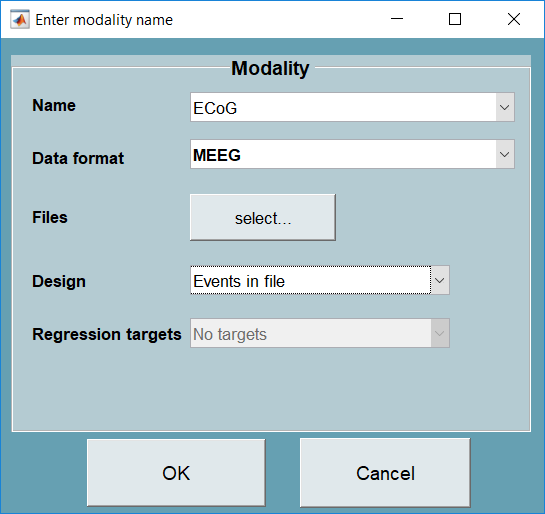
\includegraphics[scale=0.6]{images/Tutorial/v3/semi_simulated_ecog/ecog_gui_specify_modality_2.png}
		  \captionsetup{width=0.9\linewidth}
	\captionof{figure}{`Specify modality' GUI for MEEG.}
	\label{fig:ecog_gui_specify_modality_2}
\end{minipage}%
	\begin{minipage}[b][8cm][b]{0.5\textwidth}
  \centering
		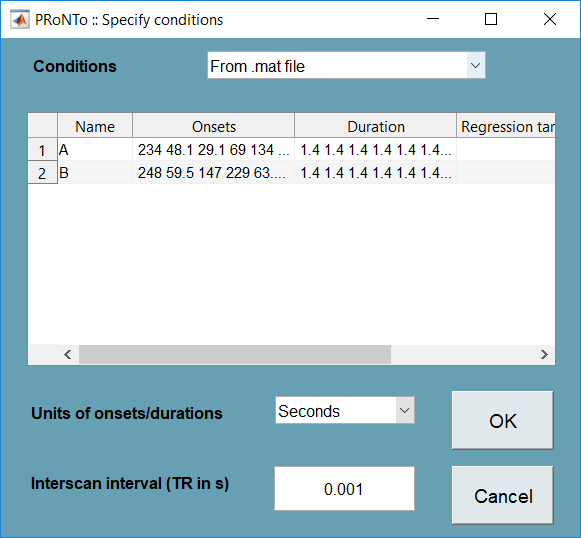
\includegraphics[scale=0.6]{images/Tutorial/v3/semi_simulated_ecog/ecog_gui_specify_modality.png}
		\captionsetup{width=0.9\linewidth}
	\captionof{figure}{`Specify conditions' GUI.}
	\label{fig:ecog_gui_specify_modality}
	\end{minipage}
\end{figure}

\item After clicking `OK' on both windows, you can save the data into a PRT.mat in the directory of your choice, and also review the data, either prior to saving them through the `Review' button in the `Data \& Design' window, or after saving them, using the `Review data' button in PRoNTo's main window.

\end{itemize}

As we can see in figure \ref{fig:ecog_gui_review_data}, we have one subject in one group that contains one modality (ECoG). There are 2 conditions (A and B). The `selected scans' reflect the `good' epochs, while the `discarded scans' reflect the epochs marked as `bad' in the SPM file.

\begin{figure}[!h]
  \centering
		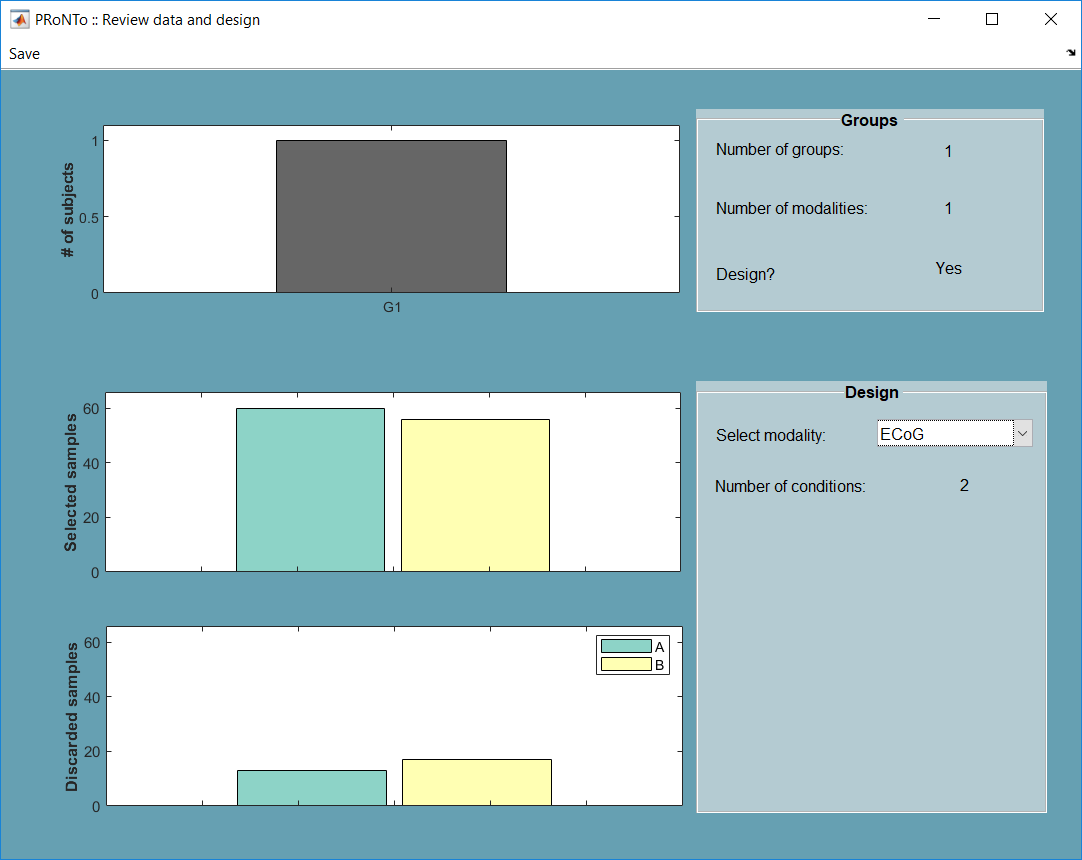
\includegraphics[scale=0.55]{images/Tutorial/v3/semi_simulated_ecog/ecog_gui_review_data.png}
	\caption{`Review data' GUI.}
	\label{fig:ecog_gui_review_data}
\end{figure}


%------------------------------------------------------------------

\subsection{Prepare feature set}
\label{sssec:feature_set_semisim_gui}


This step is probably the most different from all other new functionalities in v3. It reflects the different dimensions of the data and allows to `play' on them. Click on `Prepare feature set' in the main window and load the PRT.mat. As there is only one modality of type MEEG, the corresponding MEEG modality window will be launched directly. There are 3 main panels, corresponding to the 3 dimensions an MEEG file can have:
\\

\noindent \textbf{Channels:}

\begin{itemize}
\item The list of channels is displayed on the left panel, as unselected. To add a channel to the feature set, click on it. It will then appear on the right panel. Alternatively, you can select `All' channels or all `Good' channels. On Windows OS, the `bad' channels appear in red in the list.

\item Average signal over channels: this option will average the signal over all selected channels. This might be useful to obtain an average trace across a specific region of interest.

\item One kernel per channel: whether to build one kernel per channel (ticked) or not. This option corresponds to building an atlas with each channel as a `ROI'.
\end{itemize}

\noindent \textbf{Time points:}

\begin{itemize}
\item Similarly, the time window is displayed and can be amended. When entering a value in ms, PRoNTo will identify the closest corresponding time point.

\item The signal can be averaged across all selected time points.

\item One kernel can also be built, either per time point or per sub-windows of XX ms (user-specified). PRoNTo does not discard kernels with less than a few time points, so to avoid big imbalances in the feature numbers across kernels you should ensure you provide the right window end. For example if you want to have 100ms subwindows between -100 and 1100ms, the end time point should be 1099ms, otherwise a kernel with only one time point will be created (see batch tutorial below for example).
\end{itemize}

\noindent \textbf{Frequencies:}

\begin{itemize}

\item Similar to time points, the range of frequency bins included in the data can be viewed and specific sub-ranges selected.

\item The data can be averaged over a frequency band, as specified above. This is useful to test multiple frequency bands without having to manually perform the averages as a pre-processing step.

\item A kernel can also be built on each frequency bin.
\end{itemize}

\noindent Note 1: Dimensions that are not present in the 1st file are greyed out and the corresponding panel cannot be accessed (e.g. frequencies in the present case).
\\
Note 2: It is not possible to use `average' and `multiple kernels' on the same dimension simultaneously.


\begin{itemize}

\item In the present case, let’s first build a simple feature set, using all `Good' channels and the time points between -100ms and 1100ms (keep in mind that the simulated window was added between 0 and 1000ms). Having explained all the above it will be quite straight forward to do so.

\begin{itemize}

\item So, after you click the `Prepare feature set' button and the main window where you define the feature set has appeared, you first need to select only the `Good' channels by clicking the `Good' button, in the `Channels' section.

\item Then you need to change the time points in the `Time points' section from -100ms to 1100ms. The window at this point should look like figure \ref{fig:ecog_gui_prepare_featureSet_1_final}.


\begin{figure}[!h]
  \centering
		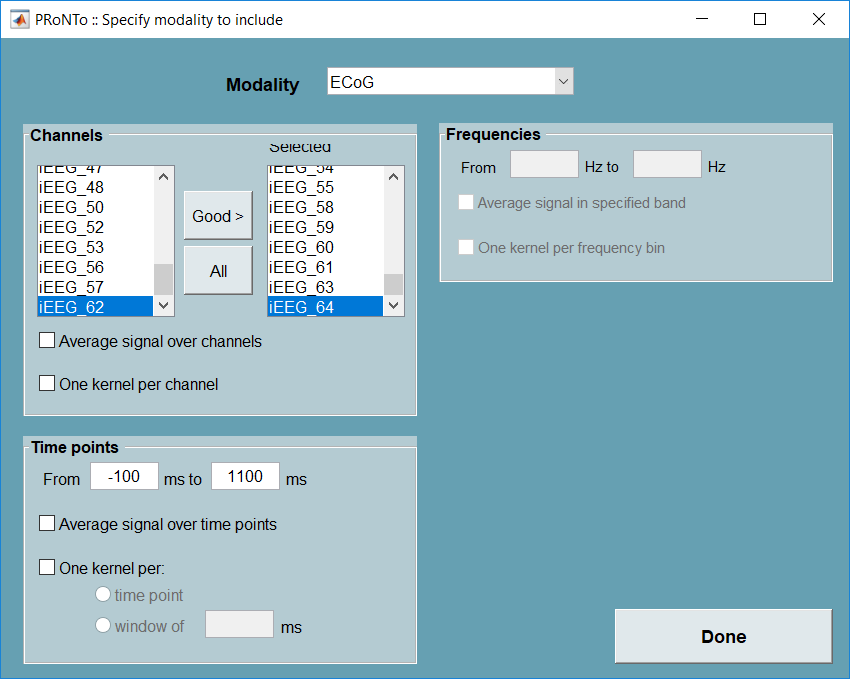
\includegraphics[scale=0.55]{images/Tutorial/v3/semi_simulated_ecog/ecog_gui_prepare_featureSet_1_final.png}
	\caption{`Specify modality to include' GUI. `All' feature set.}
	\label{fig:ecog_gui_prepare_featureSet_1_final}
\end{figure}

\item Clicking `Done' sends us to the main feature set window, where we specify the feature set name (e.g. `All').

\item Clicking on ‘Build kernel/data matrix’ builds the binary file array (as for nifti) with all the features, as well as the kernel(s) containing only the selected features. Hence, the MEEG modality window builds a second-level mask but implicitly (instead of the user specifying a file).

\end{itemize}

\item We will then repeat this operation but building one kernel per channel, for later use with L1 MKL machine, and name it `MKChans' (for Multiple Kernels on channels). As displayed in the main window, 38 kernels were built, one for each channel containing all the time points between -100 and 1100ms around onset. The final configuration of this feature set should look like figure \ref{fig:ecog_gui_prepare_featureSet_2_final}.

\end{itemize}

\begin{figure}[!h]
  \centering
		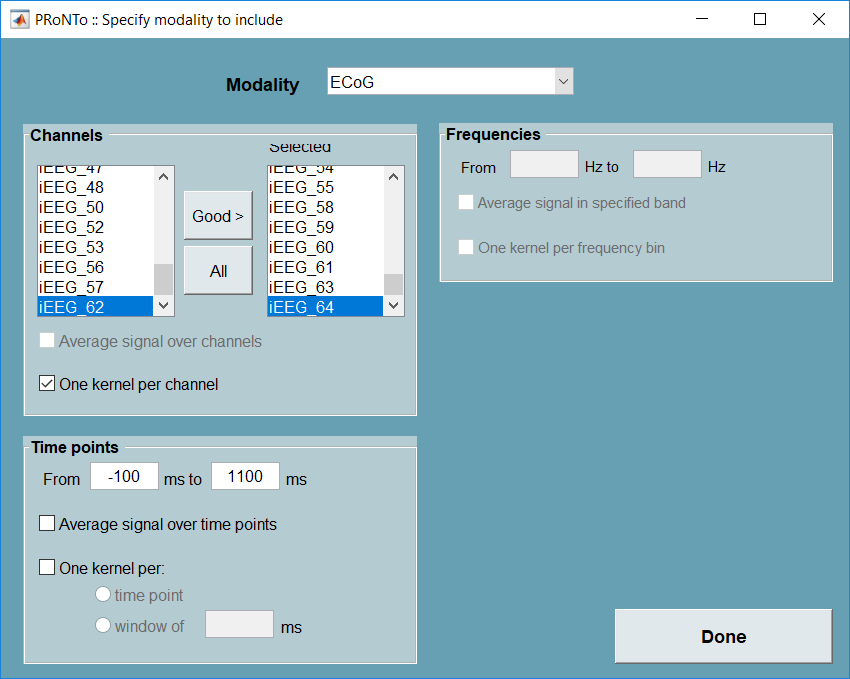
\includegraphics[scale=0.55]{images/Tutorial/v3/semi_simulated_ecog/ecog_gui_prepare_featureSet_2_final.png}
	\caption{`Specify modality to include' GUI. `MKChans' feature set.}
	\label{fig:ecog_gui_prepare_featureSet_2_final}
\end{figure}


%------------------------------------------------------------------

\subsection{Model: Specify new}
\label{sssec:specify_model_new_semisim_gui}

We can now build two models discriminating A from B: one using SVM and the other using MKL on the channels. The model specification is very similar to PRoNTo v2.1 and there is nothing specific to MEEG at this stage.

\begin{itemize}

\item For the SVM model, first choose the appropriate PRT.mat file;

\item Specify the name of our model (e.g. `SVM');

\item Choose the `All' feature set and define the classes as `A' modality A and as `B' modality B. Although the imbalance is small, we also select the `Subsample according to smallest class' option to randomly subsample 56 epochs from A to match the number of B epochs. The window should look like figure \ref{fig:ecog_gui_specify_model_specify_classes}.

\item Choose the SVM machine and optimize the hyper-parameter C (range: [0.01 0.1 1 10 100 1000]).

\item The nested cross-validation scheme (inner loop) is `k-folds on Block per Class' with k=4, meaning that we will leave approximately 25\% of A and approximately 25\% of B epochs out for testing in each fold.

\item Choose the same scheme for the outer CV with k=5.

\item Finally, mean centre the kernel and specify the model.

\end{itemize}

After you have specified everything, the final configuration should look like the one in figure \ref{fig:ecog_gui_specify_model_svm_final}.

\begin{figure}[!h]
	\centering
	\begin{minipage}[b][13cm][b]{0.5\textwidth}
  \centering
		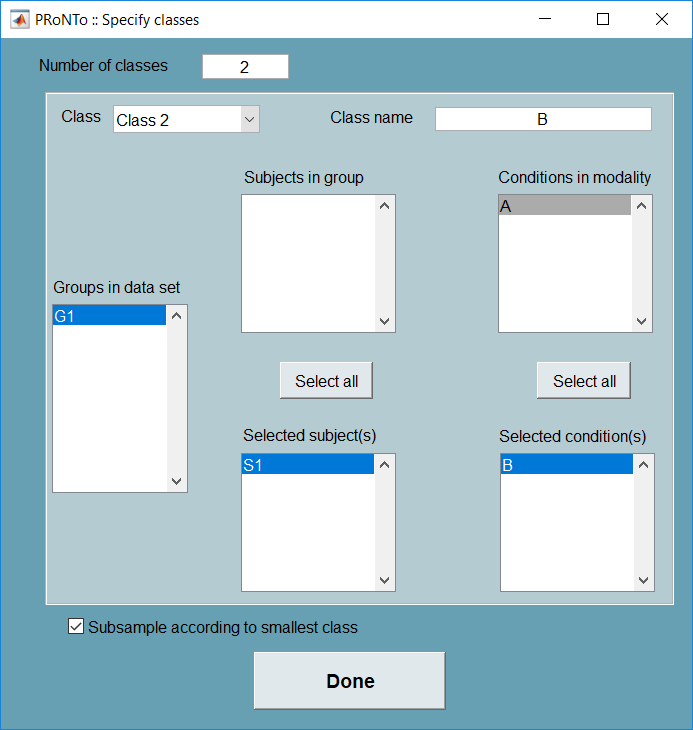
\includegraphics[scale=0.55]{images/Tutorial/v3/semi_simulated_ecog/ecog_gui_specify_model_specify_classes.png}
		  \captionsetup{width=0.9\linewidth}
	\captionof{figure}{`Specify classes' GUI.}
	\label{fig:ecog_gui_specify_model_specify_classes}
\end{minipage}%
	\begin{minipage}[b][13cm][b]{0.5\textwidth}
  \centering
		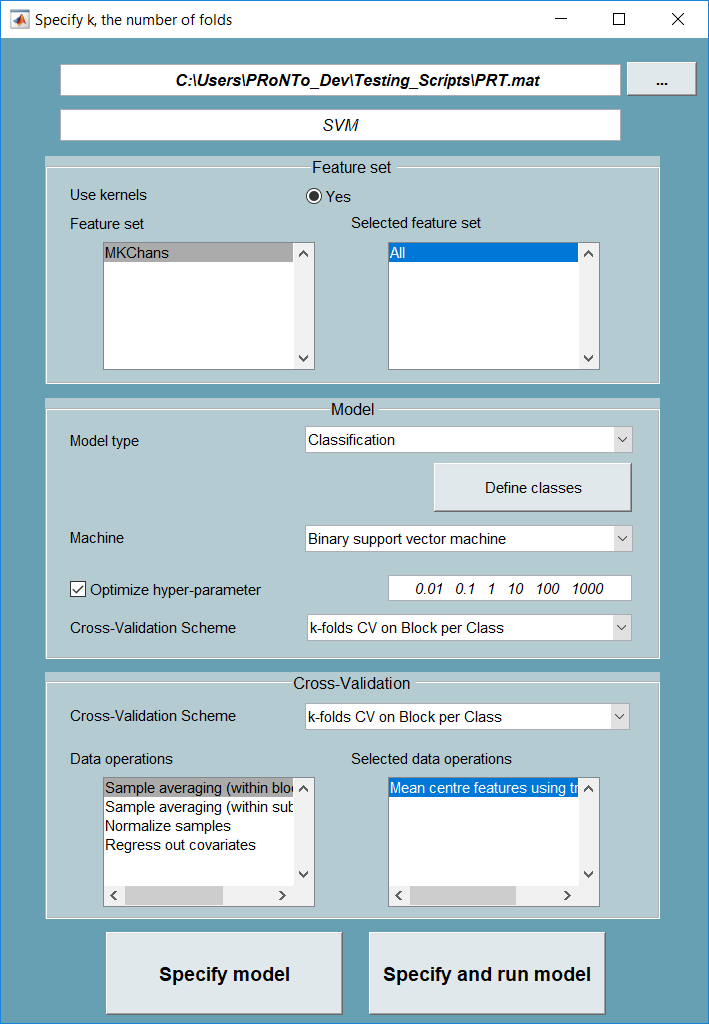
\includegraphics[scale=0.55]{images/Tutorial/v3/semi_simulated_ecog/ecog_gui_specify_model_svm_final.png}
		\captionsetup{width=0.9\linewidth}
	\captionof{figure}{`Specify model' GUI, `SVM' model.}
	\label{fig:ecog_gui_specify_model_svm_final}
	\end{minipage}
\end{figure}

%------------------------------------------------------------------

\subsection{Model: Specify from}

\begin{itemize}

\item To specify the MKL model, you need to `copy' the SVM model specifications if you want to use the same samples as the random subsample option was selected.

\item In this case, click `Specify from' and load the PRT.mat. The SVM model is loaded by default (as the first) and you can only modify the feature set, the machine (with hyper-parameter optimization) and/or the kernel operations.

\item Use the `MKChans' feature set and change the machine to `L1 Multi-Kernel Learning'.

\item Use the same hyper-parameter optimization as before;

\item But you need to add the `Normalize samples' operation. Note: as the kernels all include the same number of features (i.e. the number of time points considered), this operation could also be left out. 

\end{itemize}

After you have specified everything, the final configuration should look like the one in figure \ref{fig:ecog_gui_specify_model_mkl_final}.

\begin{figure}[!h]
  \centering
		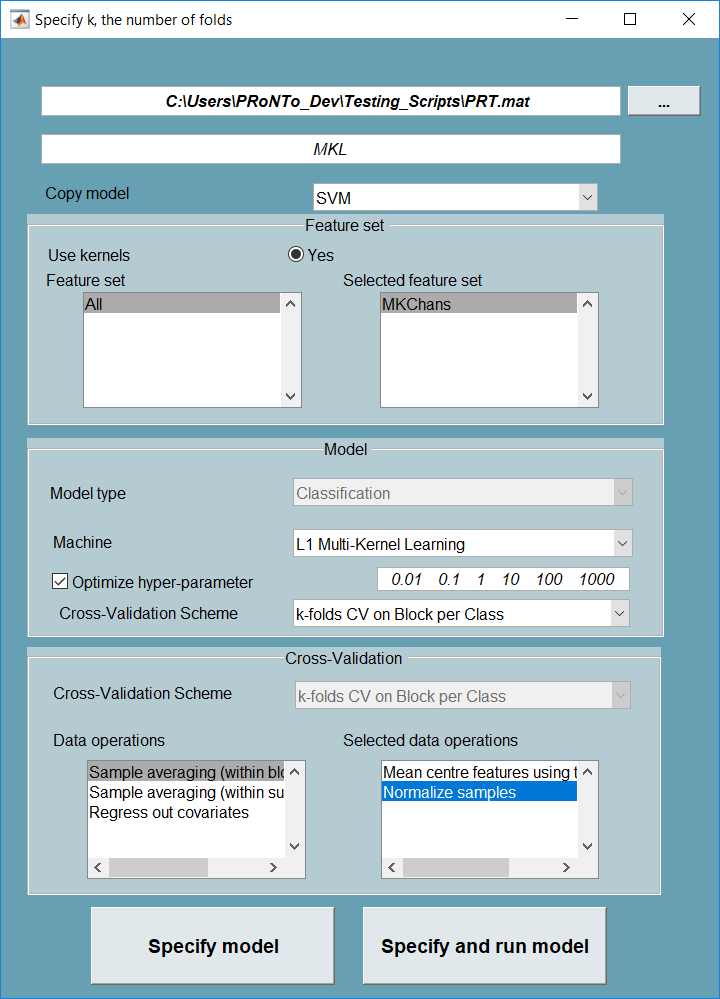
\includegraphics[scale=0.55]{images/Tutorial/v3/semi_simulated_ecog/ecog_gui_specify_model_mkl_final.png}
	\caption{`Specify model' GUI, `MKL' model.}
	\label{fig:ecog_gui_specify_model_mkl_final}
\end{figure}

%------------------------------------------------------------------

\subsection{Model: Run}

\begin{itemize}

\item  It is now time to run our models so open the `Run' module.

\item After you select the `PRT.mat' file you will see the 2 models we have created so far. You can either select and run them one by one, or you can select all and run them all together.

\item In `Permutations' select the `Perform permutation test' option with 100 repetitions. Be aware that 100 repetitions is a small number when running permutation tests, and 1000 repetitions (or even more) is a more realistic one if you want your results to have a good statistical power. You could also select the `Save permutation parameters' option, in case you wanted to perform further statistical tests.

\end{itemize}

The `Run' window should look similar to the one in figure \ref{fig:multimodal_face_gui_run_final} of Chapter \ref{sec:multimodal_face};


%------------------------------------------------------------------

\subsection{Display results}

The SVM model leads to ~93.86\% balanced accuracy, while the MKL model leads to ~95.72\%. Their AUC is however the same (1.00). It is expected that MKL performs better as only half of the good channels contain signal of interest while the other half only contains noise. The results of the `SVM' model are shown in figure \ref{fig:ecog_gui_display_results}.

\begin{figure}[!h]
  \centering
		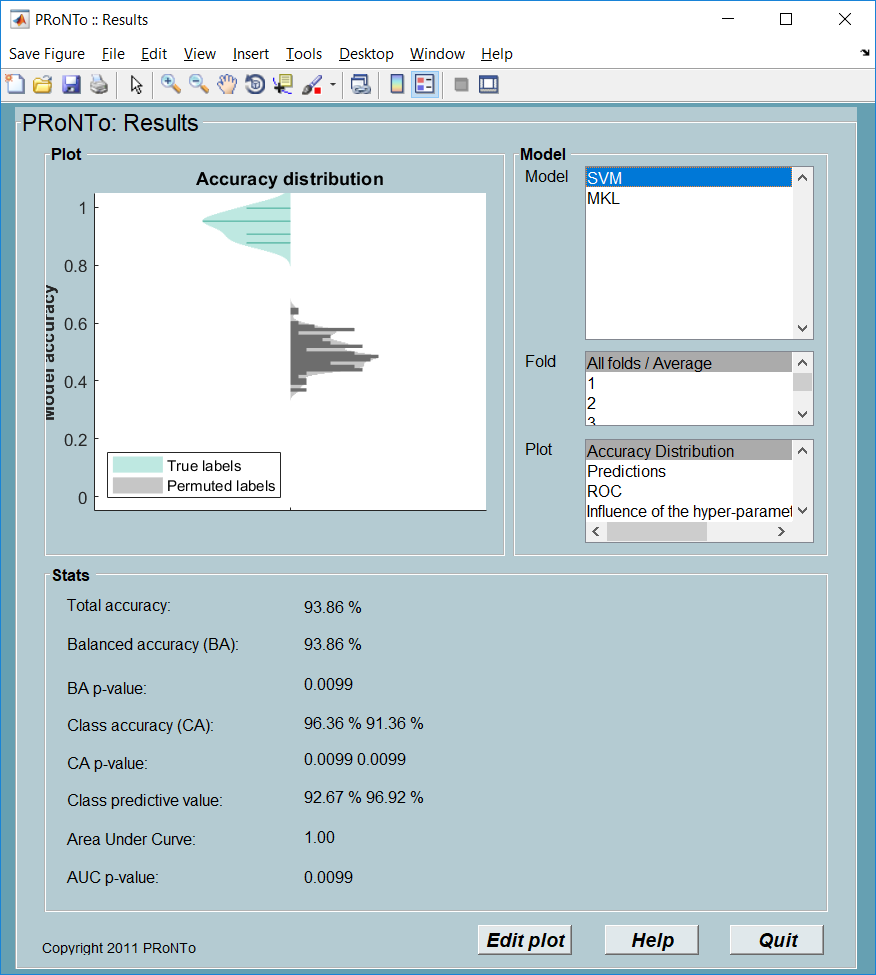
\includegraphics[scale=0.55]{images/Tutorial/v3/semi_simulated_ecog/ecog_gui_display_results.png}
	\caption{`Display results' GUI..}
	\label{fig:ecog_gui_display_results}
\end{figure}

%------------------------------------------------------------------

\subsection{Compute weights}

\begin{itemize}

\item We can now build the weights for the SVM model. In this case, select the PRT.mat, the SVM model and leave the other options as default. Please note that weight summarization is not available for MEEG data. A new file, in MEEG format, will be built containing the weights per feature. It will have the same dimensions as the input file but contain NaN where the second-level masks did not overlap with the data (i.e. the features not selected at the feature step stage).

\item Repeat the operation for the MKL model but this time tick the `Compute average/kernel weight per region'. Two images are then built: one with weights per feature, one with weight per kernel. Again, the dimensions are identical to the dimensions of the input file.

\end{itemize}

%------------------------------------------------------------------

\subsection{Display weights}

The weight display for MEEG is very basic, just a color-coded 2D matrix if there are 2 dimensions in the file (3D files are not displayed). We refer the user to SPM (or other software after conversion) for more advanced plotting.
\\

The weights for the SVM model are displayed in the following figure. As we can see in figure \ref{fig:ecog_gui_display_weights_svm}, channels are quite consistently either positive or negative. On the other hand, for the MKL model some channels have no contribution, as shown in figure \ref{fig:ecog_gui_display_weights_mkl_voxel}.
\\

\begin{figure}[!h]
  \centering
		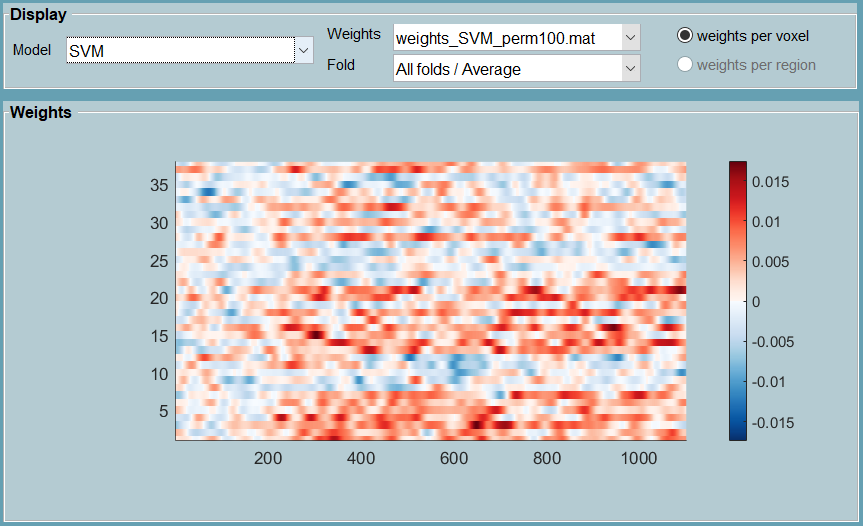
\includegraphics[scale=0.55]{images/Tutorial/v3/semi_simulated_ecog/ecog_gui_display_weights_svm.png}
	\caption{`Display weights' GUI. `SVM' model.}
	\label{fig:ecog_gui_display_weights_svm}
\end{figure}

\begin{figure}[!h]
  \centering
		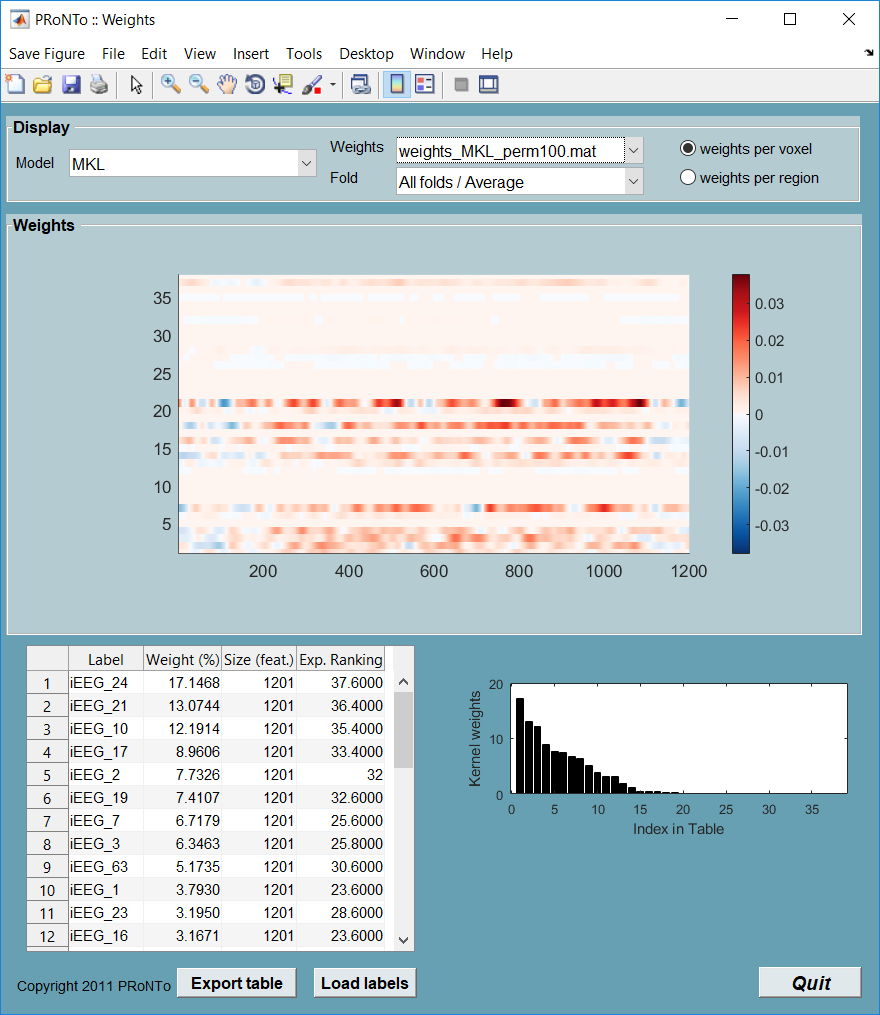
\includegraphics[scale=0.55]{images/Tutorial/v3/semi_simulated_ecog/ecog_gui_display_weights_mkl_voxel.png}
	\caption{`Display weights' GUI (per voxel). `MKL' model.}
	\label{fig:ecog_gui_display_weights_mkl_voxel}
\end{figure}

The weights per regions can also be displayed and the table of `region' (here channels) contributions is shown along a histogram depicting the sparsity of the solution. As we can see from figure \ref{fig:ecog_gui_display_weights_mkl_region}, interestingly, the histogram shows that around half of the channels have a contribution to the model (21 channels out of 38 on average across all folds).

\begin{figure}[!h]
  \centering
		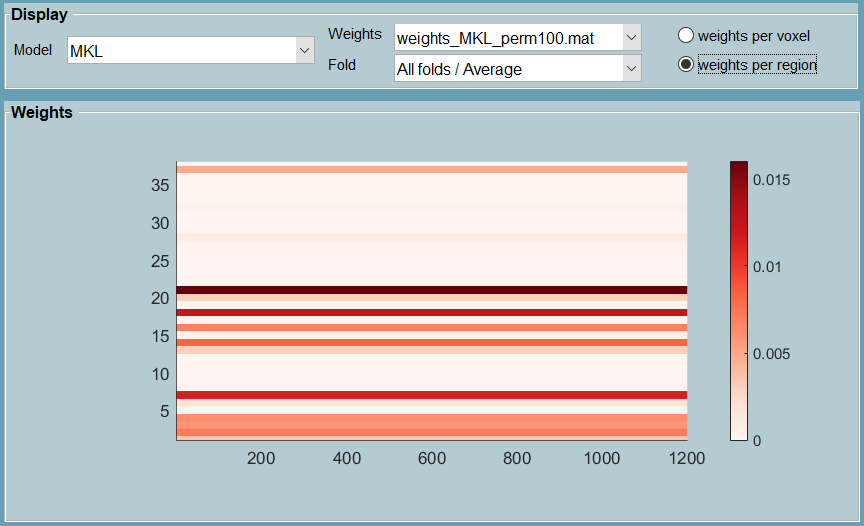
\includegraphics[scale=0.55]{images/Tutorial/v3/semi_simulated_ecog/ecog_gui_display_weights_mkl_region.png}
	\caption{`Display weights' GUI (per region). `MKL' model.}
	\label{fig:ecog_gui_display_weights_mkl_region}
\end{figure}

%==================================================================




%==================================================================

\section{Batch analysis}

In the Batch analysis of this tutorial we are not going to fully replicate the GUI analysis, so if one is not yet familiar with the Batch analysis, he/she should first go through the previous tutorials that are much more detailed.

%------------------------------------------------------------------

\subsection{Data \& Design}
\label{sssec:data_and_design_semisim_batch}


\begin{itemize}
\item Select a `batch' subfolder to write the results.
\item Add a group, `G1'.
\item Add a subject, `S1'.
\item Add a modality `ECoG'.

\begin{itemize}
\item Specify the modality type as `MEEG'.
\item The interscan interval as the sampling interval (here 0.001s).
\item Select the file
\item Under `Data \& Design', select `Events in MEEG file'. Note: this option is not selected by default as in the GUI, because the batch is agnostic of the user choices.
\item No regression targets/covariates.
\end{itemize}

\item In `Masks' add a modality, specify the name (`ECoG'), which needs to be exactly the same as the original name of the modality and finally set the data format to `MEEG'. All the important information is assumed to be already included in the MEEG file, so there is no need to specify a mask here.
\end{itemize}


After you have specified everything, the final configuration should look like the one in figure \ref{fig:ecog_batch_data_and_design_final}.

\begin{figure}[!h]
  \centering
		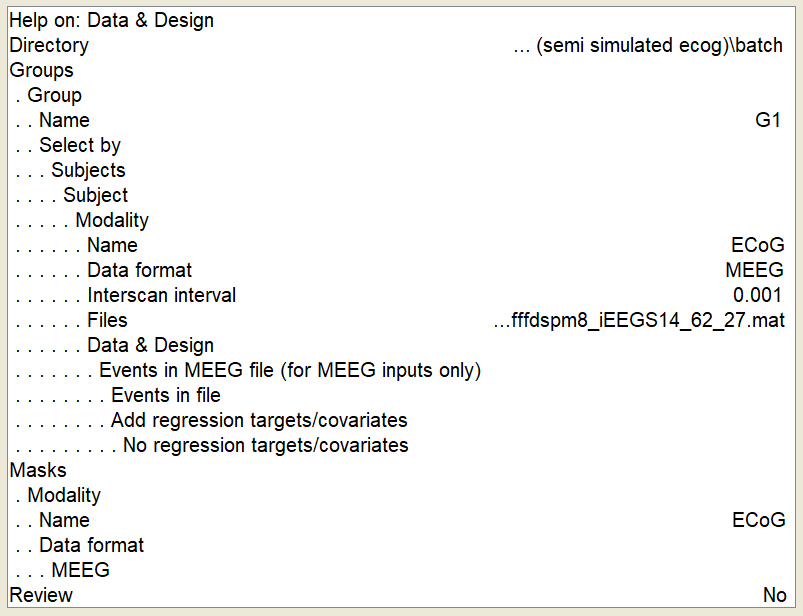
\includegraphics[scale=0.55]{images/Tutorial/v3/semi_simulated_ecog/ecog_batch_data_and_design_final.png}
	\caption{`Data \& Design' module in {\tt matlabbatch}.}
	\label{fig:ecog_batch_data_and_design_final}
\end{figure}

%------------------------------------------------------------------

\subsection{Feature set / Kernel}
\label{sssec:feature_set_semisim_batch}

In this step, we will specify a feature set for our ECoG modality. This time however we will specify a model with multiple kernels to be built at the channel level, as well as for subwindows of 100ms in our window of interest, and see how it performs compared to the models we built in the GUI analysis.

\begin{itemize}
\item First load the PRT.mat file, or create a dependency with the previous step (`Data \& Design).
\item Give a name to the feature set, e.g. `MKLChanstp'.
\item Choose the Data format as `MEEG' and add a new modality.

\begin{itemize}
\item Name the modality `ECoG' as defined in the previous step (`Data \& Design).
\item \textbf{Channels:} delete the `All' selected by default and replace it with the `New: Channel file' option. Choose the file `Good\_channels.mat' provided with the data set. This file contains the labels (in a cell array) of all the channels marked as `good' during preprocessing. The channel selector is the same as SPM. Please refer to SPM’s help for more details. Finally choose `Yes' in the `Multiple kernels' option under channels.

\item \textbf{Time points:} Specify the time window as [-100 1100]. Select `Multiple kernels' under time points and select `One kernel per time window', entering 100ms as the time window to consider for each kernel. Please note: this will create 13 kernels, from -100 to -1, 0 to 99, 100 to 199, from 200 to 299, … plus one kernel comprising the last 1100ms time point. For balanced kernels, please specify the end of your global time window (here 1100) as the end time point desired minus your sampling interval in ms (here 1). So in that case the end of your global time window would be at 1099ms.
\end{itemize}
\item Leave all the rest of the options at their defaults.
\end{itemize}

After you have specified everything, the final configuration should look like the one in figure \ref{fig:ecog_batch_prepare_featureSet_final}.

\begin{figure}[!h]
  \centering
		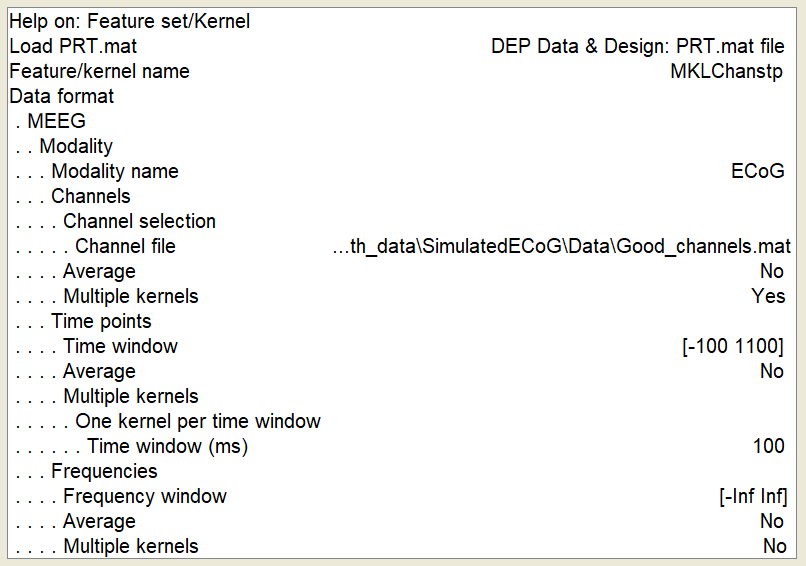
\includegraphics[scale=0.55]{images/Tutorial/v3/semi_simulated_ecog/ecog_batch_prepare_featureSet_final.png}
	\caption{`Feature set / Kernel' module in {\tt matlabbatch}.}
	\label{fig:ecog_batch_prepare_featureSet_final}
\end{figure}

%------------------------------------------------------------------

\subsection{Model: Specify new}

\begin{itemize}

\item Specify a new model (named `sMKLChanstp') that accesses your PRT.mat and choose the `MKLChanstp' feature set.

\item As in previous versions, define 2 classes, based on conditions A and B (subsampling to match the least represented class), and choose the `L1 Multi-Kernel Learning' machine.

\item As this is a within-subject design, we can use the `k-folds on block per class' cross-validation, for hyper-parameter optimization (inner loop) as well as for model performance evaluation (outer loop). Choose (arbitrarily) k=4 for the nested CV (inner loop) and k=5 for the outer CV (outer loop). As the kernels do not include the same number of features, it is important to add the ‘Normalize samples’ operation. For a more detailed way of inputting all the options and  parameters the reader is referred to Chapter \ref{sec:multimodal_face} in the parts regarding the MEEG data format.

\end{itemize}

After you have specified everything, the final configuration should look like the one in figure \ref{fig:ecog_batch_specify_model_final}.

\begin{figure}[!h]
  \centering
		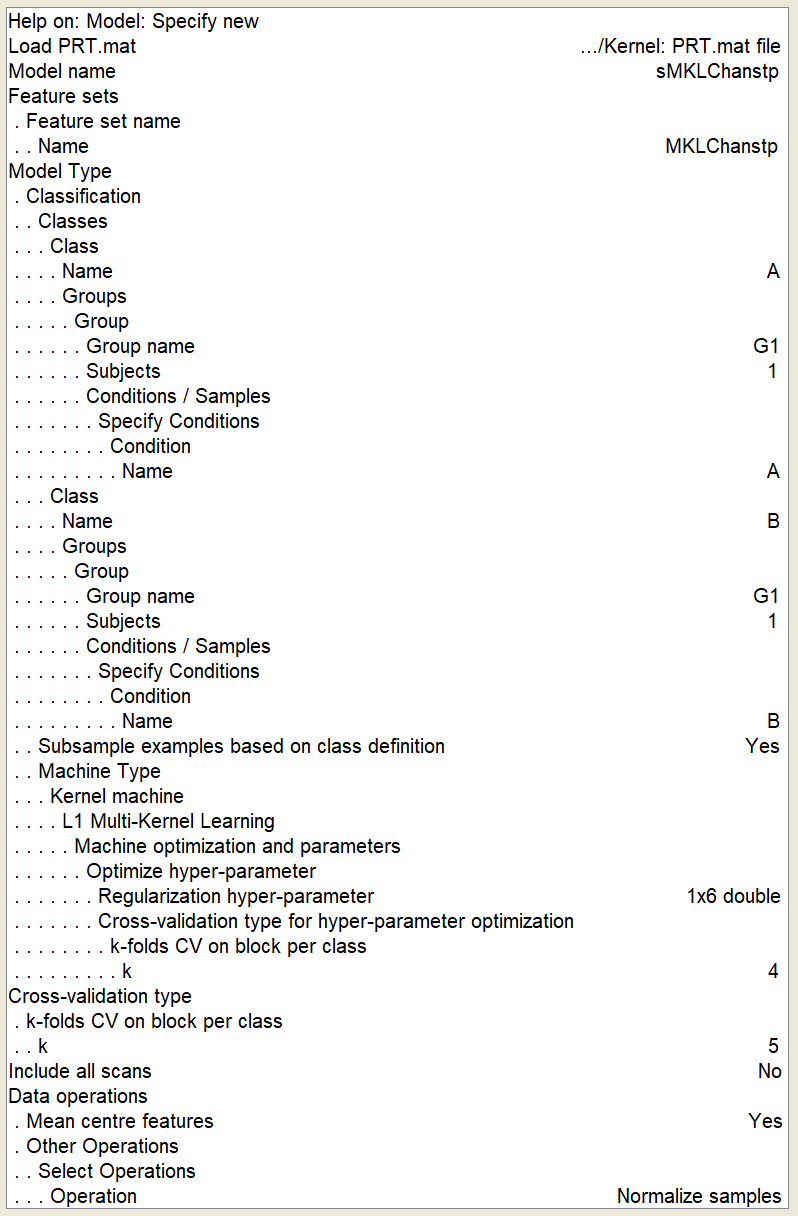
\includegraphics[scale=0.55]{images/Tutorial/v3/semi_simulated_ecog/ecog_batch_specify_model_final.png}
	\caption{`Model: Specify new' module in {\tt matlabbatch}.}
	\label{fig:ecog_batch_specify_model_final}
\end{figure}


%------------------------------------------------------------------

\subsection{Model: Run}


The `Run model' is the same as in previous PRoNTo versions. Simply load your PRT, type the name of the model as chosen in the previous step and specify whether you want to do permutation test or not (along with its options). After you have specified everything, the final configuration should look like the one in figure \ref{fig:ecog_batch_model_run}.

\begin{figure}[!h]
  \centering
		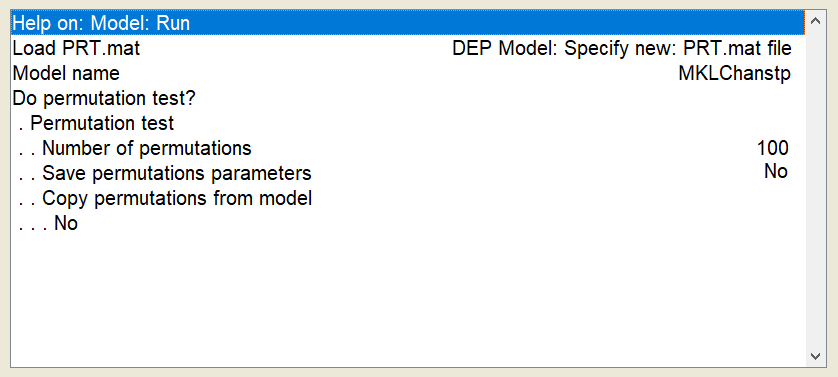
\includegraphics[scale=0.55]{images/Tutorial/v3/semi_simulated_ecog/ecog_batch_model_run.png}
	\caption{`Model: Run' module in {\tt matlabbatch}.}
	\label{fig:ecog_batch_model_run}
\end{figure}


%------------------------------------------------------------------

\subsection{Display results}


In the `Display Results' GUI in figure \ref{fig:ecog_batch_display_results}, we see that this model does not perform as well as the previous channel MKL model that we defined on the GUI analysis. % However, the difference in model accuracy is small and the standard deviation of this model is smaller, making it more stable across folds.

\begin{figure}[!h]
  \centering
		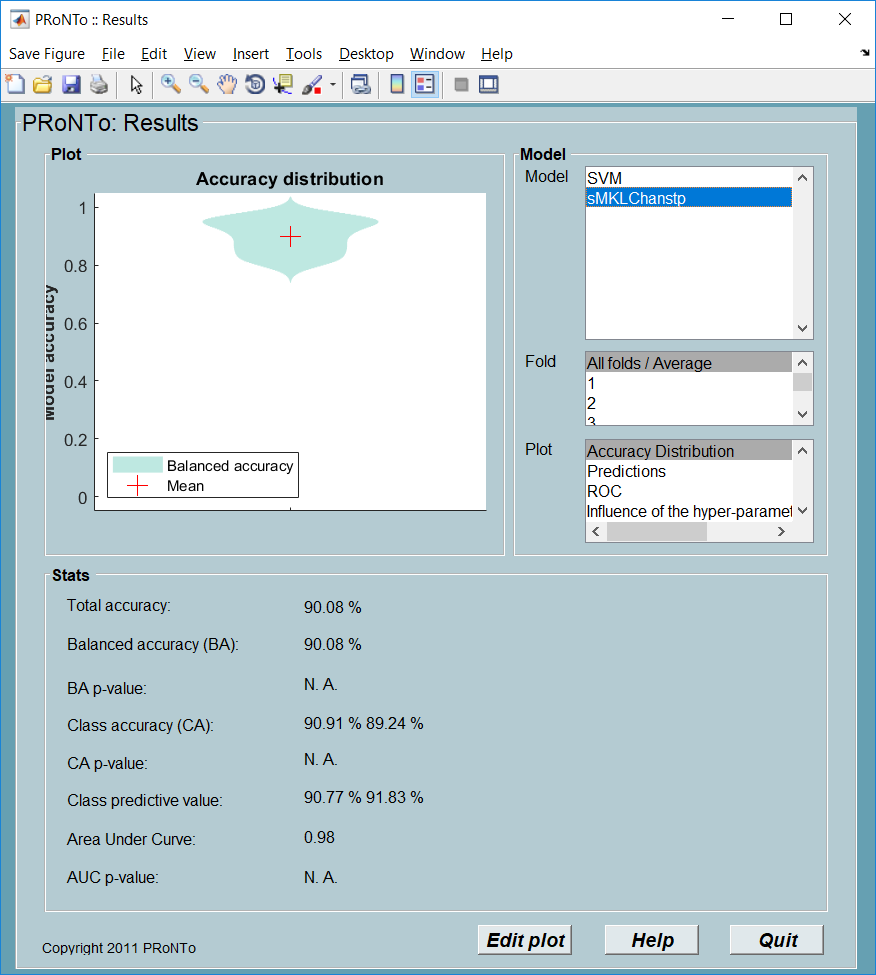
\includegraphics[scale=0.55]{images/Tutorial/v3/semi_simulated_ecog/ecog_batch_display_results.png}
	\caption{`Model: Run' module in {\tt matlabbatch}.}
	\label{fig:ecog_batch_display_results}
\end{figure}

%------------------------------------------------------------------

\subsection{Compute \& Display weights}

In this last (optional) step, we’re interested in the kernel contributions. More specifically, is the discrimination distributed in time or not? In the present case, we know the ground truth as from the simulated signal, the discrimination is uniform in the [0 1000]ms time window. It is hence interesting to look at kernel contributions to see if this information from the simulated signal was properly recovered.

\begin{itemize}

\item To this end, select `Compute weights' and load the PRT.mat.

\item Specify the model name as before and select the `Build weights per region' option, leaving the `Load atlas' as it is (blank). PRoNTo will automatically access the atlas defined at the feature set step if no atlas is specified.

\end{itemize}

After you have specified everything, the final configuration should look like the one in figure \ref{fig:ecog_batch_compute_weights}.
\\

\begin{figure}[!h]
  \centering
		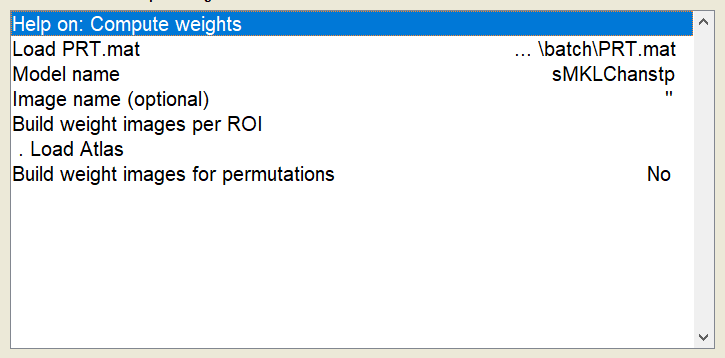
\includegraphics[scale=0.55]{images/Tutorial/v3/semi_simulated_ecog/ecog_batch_compute_weights.png}
	\caption{`Compute weights' module in {\tt matlabbatch}.}
	\label{fig:ecog_batch_compute_weights}
\end{figure}

In the `Display Weights' window, click on the model and select `Weights per region'. You will see the table of kernel contributions for each channel and time window (referred to by their starting time point in ms).
\\

As we can see in figure \ref{fig:ecog_batch_display_weights}, the MKL model mostly identifies time windows within the [0 1000]ms window of simulated signal. However, the MKL only provides a sparse solution, i.e. it does not recover all time windows that have discrimination information in the A vs B classification.

\begin{figure}[!h]
  \centering
		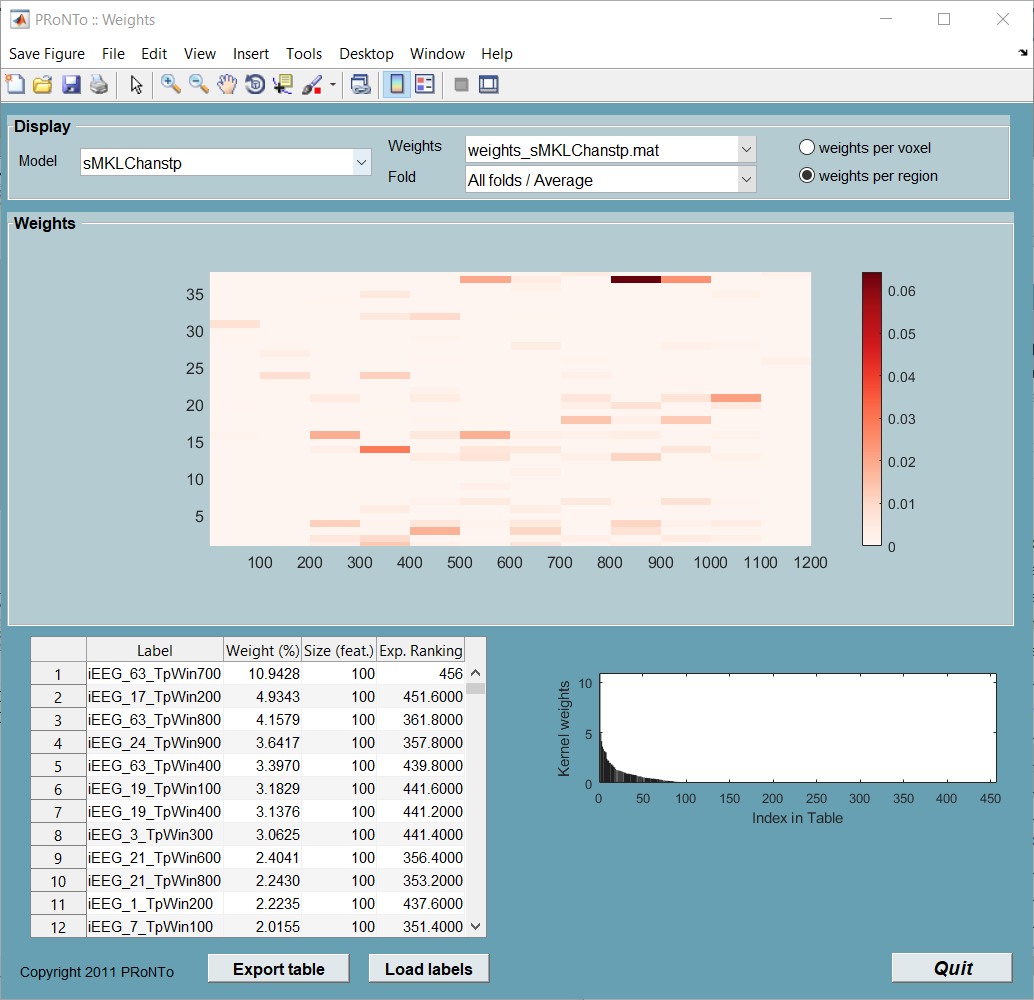
\includegraphics[scale=0.55]{images/Tutorial/v3/semi_simulated_ecog/ecog_batch_display_weights.png}
	\caption{`Display weights' GUI.}
	\label{fig:ecog_batch_display_weights}
\end{figure}



